% Created 2023-05-25 jeu. 17:31
% Intended LaTeX compiler: pdflatex
\documentclass[11pt]{article}
\usepackage[utf8]{inputenc}
\usepackage[T1]{fontenc}
\usepackage{graphicx}
\usepackage{grffile}
\usepackage{longtable}
\usepackage{wrapfig}
\usepackage{rotating}
\usepackage[normalem]{ulem}
\usepackage{amsmath}
\usepackage{textcomp}
\usepackage{amssymb}
\usepackage{capt-of}
\usepackage{hyperref}
\author{Clément Morand}
\date{\today}
\title{Experiments for validating our tool}
\hypersetup{
 pdfauthor={Clément Morand},
 pdftitle={Experiments for validating our tool},
 pdfkeywords={},
 pdfsubject={},
 pdfcreator={Emacs 27.1 (Org mode 9.3)}, 
 pdflang={English}}
\begin{document}

\maketitle
\tableofcontents

In order to validate our tool we first need to conduct some
experiments to ensure that it produces results consistent with the
state of the art. Our tool estimates manufacture impacts of the
hardware used and energy consumption over the usage duration (typically
during the training phase of a model). We therefore want to test those
two parts. 
Firstly, we will present experiments aimed at testing the
estimates for the dynamic energy consumption (and the results we will
present will therefore focus only on the energy consumption estimated
and on the Carbon footprint induced by this energy consumption). These experiments will
start in section \ref{sec:ga} by reproducing the same exact results as the
Green Algorithms tool, by first choosing a scenario were we know that
our tool and Green Algorithms use the same data. Then, in section
\ref{sec:bannour, sec:jay} we will focus
on reproducing results presented in the two surveys of existing tools
(\cite{Bannours2021evaluating} and
\cite{Jay2023experimental}). Finally, in sections \ref\{sec:dinarelli,
sec:catta, sec:strubell\} we will try to reproduce results
obtained with a different method than the one used by our tool. This
will be done by trying to reproduce results from
\cite{Dinarelli2022toward}, \cite{Cattan2022benchmarking} and
\cite{Strubell2019energy}. We chose those articles because they all
use a different tool (even if measures presented in these three
articles are based on the \gls{RAPL} and \gls{NVLM} tools), because we
were able to contact the authors of
\cite{Dinarelli2022toward,Cattan2022benchmarking} to obtain further
details about the hardware configuration they use ; Because
\cite{Cattan2022benchmarking} presents results about the inference
phase of models which is a phase that is rarely studied and because
\cite{Strubell2019energy} was the paper that made NLP researchers
consider the impacts of the models they produced.
Secondly, in section \ref{sec:manufacture_comparison} we will compare the results our tool produces with \gls{LCA}
results produced by Dell about the impacts of the servers they
sell. This will allow us to validate the estimations of embodied
impacts our tool generates.
Finally, in section \ref{sec:bloom} we will try to reproduce the results from
\cite{Luccionni2022estimating}, this step is really important because
this paper conducts an analysis of the global warming potential
induced by the Bloom model. This analysis takes into account embodied
emissions and we use figures they present to define the default
dynamic ratio our tool uses.

\section{Checking that we can get the same dynamic consumption estimate as Green Algorithms}
\label{sec:org30bd020}
\label{sec:ga}
To do a first sanity check, we verify that we are able to reproduce
the same results as GA on the dynamic consumption part :

We choose a configuration that we know is available in both databases
(GA version 2.2 at the time of this experiment):
\begin{itemize}
\item 1 CPU A8-7680 (4 cores)
\item 1 GPU NVIDIA GTX 1080 Ti
\item 64 GB Memory

\item Use time of 12h 0min
\item no PUE / dynamic ratio
\item carbon intensity of France is used (51.28 g CO\textsubscript{2} e/kWh)
\end{itemize}

We are using Green Algorithms v2.2
for an expected result of 196.32g of CO\textsubscript{2} e and 3.83 kWh of dynamic
consumption (this \href{http://calculator.green-algorithms.org//?runTime\_hour=12\&runTime\_min=0\&appVersion=v2.2\&locationContinent=Europe\&locationCountry=France\&locationRegion=FR\&PUEradio=Yes\&PUE=1\&coreType=Both\&numberCPUs=4\&CPUmodel=A8-7680\&numberGPUs=1\&GPUmodel=NVIDIA\%20GTX\%201080\%20Ti\&memory=64\&platformType=localServer}{link} should in theory get you to the page with this
exact setup and results but it seems like GA sharing feature is broken right
now).

If we now run the experiment with our tool :
we see that we indeed obtain the same results of 196gCO\textsubscript{2} e and 3.83
kWh of dynamic energy consumption.

\section{replicating results from \cite{Bannour2021evaluating}}
\label{sec:orgef0377d}
\label{sec:bannour}
In order to replicate results, we first need to gather some
information about the hardware configuration used to run the
experiments. Then, we will face the challenge of inconsistencies in the
data presented in the paper. Finally, we will be able to run
experiments that give the same energy consumption estimates as those
presented in the paper.

\subsection{detailing the Hardware configurations}
\label{sec:org36bd262}
The authors provided us with information about the hardware
configurations used to run  the experiments. 

the facility setup is the \href{https://doc.lab-ia.fr/}{LaBia} cluster. We can see that the only nodes using a
20 core CPU are: n[101-102]:

\begin{itemize}
\item 2 x Intel Xeon Gold 6148 20 cores / 40 threads @ 2.4 GHz (Skylake)
\item 384 GiB of RAM
\item 4 x NVIDIA Tesla V100 with 32 GiB of RAM (NVLink)
\end{itemize}

using 32 GB of RAM and not the full 384.

The lab server on the other hand is the Segur machine, using one GTX 1080 Ti with 11GB of memory.
it is a Dell PowerEdge R730 with 2 GTX 1080 Ti, 2 Intel Ben E5-2620
v4 CPU and 125 GB memory (only 11 of which are requested).

while we do not have the Intel Xeon Gold 6148 in our CPU database, we
can see on \href{https://www.intel.fr/content/www/fr/fr/products/sku/120489/intel-xeon-gold-6148-processor-27-5m-cache-2-40-ghz/specifications.html}{Intel's website} that it has a \gls{TDP} of 150W, was released in
2017 with a process of 14nm with the Skylake architecture, this is
sufficient information to add one entry to our database, knowing the
information about the Skylake architecture from \href{https://en.wikichip.org/wiki/intel/microarchitectures/skylake\_(server)}{WikiChips}. 

\subsection{Problems with the provided data}
\label{sec:orgc674b7a}

Results presented in the paper do not seem coherent from one table to
the other (tables 3 and 4). If we try to convert from energy consumption to carbon
emissions using the presented carbon intensity of 39 gCO\textsubscript{2} e/kWh we do
not at all find the same results as the ones presented.
For instance, for the first method (Yu2020) for the French Press
benchmark, it is indicated 1.38kWh consumption and 350.15g CO\textsubscript{2} e.

We can see that if we are to use the presented carbon intensity, we
get emissions of 
\texttt{53.8} gCO\textsubscript{2} e for a 1.38kWh energy consumption. This is
really far from the 350 gCO\textsubscript{2} e presented in the paper.

\subsubsection{Trying to understand the problem}
\label{sec:orgab4e0bd}

Let us check if the factor to convert from table 4 to table 3 is
constant.
If it is, it would maybe explain the problems. When filling the table
the authors might have miss-clicked on the location and the Carbon
Intensity used would just be the one of another country.

We obtain results around 250 gCO\textsubscript{2} e/kWh with some non negligible
variations (The smallest conversion factor is of 191.5 gCO\textsubscript{2} e/kWh
while the highest is of 283.5 gCO\textsubscript{2} e/kWh)

according to GA's v2.2 database, this carbon intensity of around 250gCO\textsubscript{2}
e/kWh would approximately correspond to Lithuania's one. According to
the version 1.1 of the data (version seemingly used in the article),
the closest one would be Hungary.

Still, we can observe quite important variations in carbon intensity
to convert from the presented energy consumption to the presented
carbon emissions, this would tend to infirm the hypothesis of just an
error of selection in the carbon intensity used. 

Even if there are obviously problems with the presented data, we still
want to try and replicate the presented results. Indeed, if the data
is flawed only in the table presenting the energy consumption or only
in the table presented the carbon footprint, we might be able to
reproduce the results of one of the tables (i.e. either the
consumption or the carbon footprint)

\subsection{experiments}
\label{sec:org52e3eca}
It is said that the default \gls{PUE} used is 1.67. In order to replicate
the results, and even if the dynamic ratio and the \gls{PUE} do not have the
same meaning. Since they are both used in the same way we will use a
dynamic ratio of 1.67

we can see in \href{https://github.com/GreenAlgorithms/green-algorithms-tool/blob/master/data/latest/TDP\_gpu.csv}{the latest version of Green Algorithms' GPU TDP database}
that they have a \gls{TDP} value of 300W for a Tesla V100 GPU whereas we
have a \gls{TDP} of 250W for the same card in our database. In order to see
if we can replicate the same consumption and see the difference
resulting from this data-point inconsistency we will try two
versions. One with a V100 and one with a card with a \gls{TDP}
of 300W in our database: the NVIDIA A100 PCIe 80 GB. This will of
course also impact the manufacture impacts but we are here only focusing on
reproducing the same direct impacts

\begin{table}[htbp]
\caption{Comparison of our estimates with the expected results for the different NER experiments, the columns 'trying to match' present a scenario where we volontarily choose an  NVIDIA A100 PCIe 80 GB card to match the TDP used in Green Algorithms}
\centering
\begin{tabular}{lllrrrrrr}
Method & Task & Hardware & Expected & Estimated & Estimation & Expected & Estimated & Estimation\\
 &  &  & Energy & Energy & trying to match & Carbon & Carbon & trying to match\\
 &  &  &  &  & Facility only &  &  & Facility only\\
 &  &  & (kWh) & (kWh) & (kWh) & (gCO2e) & (gCO2e) & (gCO2e)\\
\hline
Yu2020 & French Press & Server & 1.38 & 1.16 & nan & 350.15 & 45.1 & nan\\
Yu2020 & French Press & Facility & 1.03 & 0.861 & 1.03 & 260.26 & 33.6 & 40\\
Yu2020 & EMEA & Server & 0.07 & 0.0673 & nan & 16.67 & 2.62 & nan\\
Yu2020 & EMEA & Facility & 0.06 & 0.0499 & 0.0595 & 14.31 & 1.95 & 2.32\\
Yu2020 & MEDLINE & Server & 0.08 & 0.0843 & nan & 20.68 & 3.29 & nan\\
Yu2020 & MEDLINE & Facility & 0.08 & 0.0669 & 0.0797 & 20.03 & 2.61 & 3.11\\
Ma2016 & French Press & Server & 0.41 & 0.414 & nan & 104.4 & 16.1 & nan\\
Ma2016 & French Press & Facility & 0.4 & 0.341 & 0.406 & 102.08 & 13.3 & 15.8\\
Ma2016 & EMEA & Server & 0.02 & 0.0158 & nan & 3.8 & 0.616 & nan\\
Ma2016 & EMEA & Facility & 0.02 & 0.0179 & 0.0213 & 4.99 & 0.697 & 0.83\\
Ma2016 & MEDLINE & Server & 0.02 & 0.0225 & nan & 5.57 & 0.878 & nan\\
Ma2016 & MEDLINE & Facility & 0.02 & 0.0216 & 0.0258 & 5.67 & 0.843 & 1\\
\end{tabular}
\end{table}

Table \ref{tab:bannour} presents the estimate our tool produces in
comparison with the Expected values presented in the paper. We can see that we are able to obtain the same exact energy consumption
estimates up to rounding (when we do the modifications to the inputed setup for the
facility) except for Yu2020, French Press, Server where we have a
slightly lower estimation than the one proposed in the paper.
We can also see that, as expected, the estimates we do when
considering the "real" setup are lower than the ones presented in the
paper and this can be entirely explained by the difference in \gls{TDP} in
the database.
We can also conclude that the problem in the presented data lies in
the estimates of the carbon footprint and not in the estimates of
energy consumption.


\section{replicating results from \cite{Jay2023experimental}}
\label{sec:org81b2ca4}
\label{sec:jay}
In order to replicate the results from the paper, we first need to
gather some information from the paper and its supplementary material
which is designed to allow for reproducible experiments.

\begin{itemize}
\item The hardware used is a Nvidia DGX-1 with two Intel Xeon E5-2698 v4, 512 GB of memory and 8 NVIDIA Tesla V100-SXM2-32GB.
\item The Carbon Intensity for France used in Green Algorithms V2.2 is
51.28gCO\textsubscript{2} e/kWh (\href{https://github.com/GreenAlgorithms/green-algorithms-tool/blob/master/data/latest/CI\_aggregated.csv}{latest version of Green Algorithms' Carbon
Intensity Database})
\item To convert from kWh to kJ, one must multiply the result by 3.6E+3.
\end{itemize}

we can see in \href{https://github.com/GreenAlgorithms/green-algorithms-tool/blob/master/data/latest/TDP\_gpu.csv}{the latest version of Green Algorithms' GPU TDP database}
that they have a \gls{TDP} value of 300W for an NVIDIA V100 GPU whereas we
have a \gls{TDP} of 250W for the same card in our database. As a first
version, just to see if we are able to obtain the same exact results
as those presented in the paper, we will use as GPUs a card with a \gls{TDP}
of 300W in our database: the NVIDIA A100 PCIe 80 GB.

We can also see that the CPU model used is the Xeon E5-2698 v4 with a
tdp 135. However, it isn't available in Green Algorithm, the model
used is the Xeon E5-2697 v4 with a \gls{TDP} of 145W and 18 cores.
In order to reproduce the results presented in the paper, we will use
in our setup one CPU with 40 cores, a \gls{TDP} of 324W (145/18*40) and a
die size of 9.12cm² (2*the die size of a Xeon E5-2698 v4, not relevant
for the computation of energy)

In the notebook accompanying the paper, we can see that the link explaining the configuration used for the CPU benchmarks are
exact copies of the ones for GPU benchmarks. We will therefore assume
that the CPU usage was 1 and GPU usage was 0. This configuration leads
to an energy consumption of 8.58Wh for one minute. Since this value is
strangely similar to the value of 7.58Wh/min used in the paper, we will also assume that there was a mistake when copying
results from the Green Algorithm website and therefore use the value
of 8.58Wh/min instead of the value of 7.58Wh/min to compute the
expected results.

Table \ref{tab:benchmark} present the results obtained when trying to match the expected results (same hardware setup as used for
obtaining values with Green Algorithms) and Table \ref{tab:benchmark_real_hardware} present the results obtained When using the hardware setup really used.
\begin{table}[htbp]
\caption{GPU benchmark}
\centering
\begin{tabular}{lrr}
Benchmark & Value (kJ) & Difference (kJ)\\
\hline
EP & 176.04 & -0.134\\
LU & 381.6 & -0.043\\
MG & 134.28 & -0.049\\
\end{tabular}
\end{table}

\begin{table}[htbp]
\caption{CPU benchmark}
\centering
\begin{tabular}{lrr}
Benchmark & Value (kJ) & Difference (kJ)\\
\hline
EP & 25.74 & 0\\
LU & 15.444 & 0\\
MG & 64.44 & 0.09\\
\end{tabular}
\end{table}

\begin{table}[htbp]
\caption{GPU benchmark}
\centering
\begin{tabular}{lrr}
Benchmark & Value (kJ) & Difference (kJ)\\
\hline
EP & 149.04 & -27.134\\
LU & 324.36 & -57.283\\
MG & 117 & -17.329\\
\end{tabular}
\end{table}

\begin{table}[htbp]
\caption{CPU benchmark}
\centering
\begin{tabular}{lrr}
Benchmark & Value (kJ) & Difference (kJ)\\
\hline
EP & 23.04 & -2.7\\
LU & 13.824 & -1.62\\
MG & 57.6 & -6.75\\
\end{tabular}
\end{table}

We can see that we are able to obtain results that are exactly the
same as the expected ones up to rounding errors (difference 3 orders of magnitude
lesser than the value). We can also see that even though the input
value to Green Algorithms does not exactly correspond to the hardware
setup used, the difference to the expected
results isn't too high. The difference between our estimate using
'correct' data and the expected values is around 10\% of the estimated value.
These results demonstrate the importance of inputting the right
hardware if one wants precise results.

\section{replicating results from \cite{Dinarelli2022toward}}
\label{sec:org8b83a9a}
\label{sec:dinarelli}
As for other experiments aiming at reproducing results, we first need
to gather enough information to run our 
experiments. We will also check the consistency of the results
presented in the paper. This will allow us to run our estimates.
We will focus on two results that we will try to reproduce. First the
fine tuning of the SSL model which is the most time consuming task
presented and then we will focus on the training time for the spectro
model, this should allow us to get a good overview of the results.

\subsection{Trying to find information about the hardware setup}
\label{sec:org7f2c916}

The authors gave us some insight on the hardware used for running
their experiments. Without their help, we would not have been able to
produce a single estimate. 

\subsubsection{Hardware for the fine-tuning}
\label{sec:org841f8bc}
The author said that a node from the Jean Zay supercomputer with 4 GPUs with
32GB memory was used for the fine tuning of the wave2vec model. if we look at the \href{http://www.idris.fr/jean-zay/cpu/jean-zay-cpu-hw.html\#gpu\_p13}{Idris' website} we
think that the nodes used were from the \textbf{v100-32g}, it is the only node
with matching requirements in terms of number of GPU and memory per
GPU.

these nodes have the following hardware configuration :
\begin{itemize}
\item 2 Intel Cascade Lake 6248 (20 cores at 2,5 GHz)
\item 192 GB  memory per node
\item 4 GPU Nvidia Tesla V100 SXM2 32 GB
\end{itemize}

Because we do not have the Intel Cascade Lake 6248 in our database, we
need to find some information about it. We can see on \href{https://www.intel.fr/content/www/fr/fr/products/sku/192446/intel-xeon-gold-6248-processor-27-5m-cache-2-50-ghz/specifications.html}{Intel's webpage}
that it is a processor of the Cascade Lake architecture. On \href{https://en.wikichip.org/wiki/intel/microarchitectures/cascade\_lake\#LCC\_SoC}{Wikichip},
we can see that Cascade Lake Processors use dies largely similar to
those of the \href{https://en.wikichip.org/wiki/intel/microarchitectures/skylake\_(server)\#Core}{Skylake cores}. Combining all of these pieces of
information, we can get an estimation of the details of an Intel
Cascade Lake 6248 :
\begin{itemize}
\item model: "Xeon Gold 6248"
\item manufacture date: "2019"
\item process: 14nm
\item number of cores: 20
\item die size: 694 mm² (XCC configuration)
\end{itemize}

\subsubsection{Hardware for training the models}
\label{sec:org6a939fc}

We are told that training uses only one GPU at a time and that it uses
roughly half of the time a RTX 2080 Ti and the other half a GTX 1080
Ti, to represent this, we will put the two different models in the
list of GPUs and use a 'gpu usage' of .5.
We are also told that the training uses 80 GB memory with no
additional information on the hardware used.
Since we do not know any more precise information, we will use the
default values of our tool to complete the missing pieces of information

\subsection{coherency of the results}
\label{sec:orge2628bb}

One first good news is that information are coherent with themselves.
Using the indicated (in the paper) carbon intensity of 51gCO\textsubscript{2} e/kWh
used and indicated energy consumption, we are able to find back the carbon emissions
indicated in the table. The only problem is that for table 1, it seems
that there was a translation error when filling the table. The figures
are written in the french notation with "," separating units from
decimals and not the usual ".".
For instance, if we look at the first line of table 1, we can read
a consumption of 4,473 kWh, that we can translate to 4.473 kWh.
We obtain =228.123=g CO\textsubscript{2} e, the same value as indicated in the paper.

We then only need to be able to find coherent energy consumption
values to obtain comparable results.

\subsection{Estimating energy consumption}
\label{sec:org0d1aecf}

\subsubsection{fine tuning of the SSL model}
\label{sec:org4cb1e1c}

When running an estimate of the impacts of the fine tuning, we can see that we obtain an estimate of 5.46kg CO\textsubscript{2} e for the direct
impacts and a dynamic consumption of 107 kWh, which is close to the
4.729kg CO\textsubscript{2} e and 97.720 kWh presented in the paper. The fact that
results aren't a perfect match and slightly higher than presented can
be explained by the fact that measures presented were carried out
based on a measurement tool (CarbonTracker). (results presented are
borrowed from \cite{Evain2021task} using the methodology from \cite{parcollet2021energy})

\subsubsection{Table 1}
\label{sec:org8ba3360}
We now turn our focus towards replicating the measure of impacts for
the spectro experiments presented in the Table 1 of the paper.
\begin{table}[htbp]
\caption{Comparison of our estimates with the measures presented on the spectro experiments}
\centering
\begin{tabular}{lrrrr}
model & expected & estimated & expected & estimated\\
 & power (kWh) & power (kWh) & carbon (gCO2e) & carbon (gCO2e)\\
\hline
spectro 3 steps & 4.473 & 10.1 & 228 & 517\\
spectro 2 steps & 2.989 & 6.78 & 152 & 346\\
spectro 1 step & 1.708 & 4.44 & 87 & 226\\
\end{tabular}
\end{table}

We can see that we obtain carbon emission estimates around 3 times higher than
those presented in the paper, This difference is important but results
are still in the same order of magnitude. It is expected that we obtain higher
estimates than the measurements as presented in
\cite{Jay2023experimental} but the difference could potentially be
explained by the lack of information about the GPU usage (if GPUs were
running at 30$\backslash$% capacity for instance) during training.

\section{results from \cite{Cattan2022benchmarking}}
\label{sec:org1eeb34d}
\label{sec:cattan}
This paper studies the gains and impacts of choosing to use one type
of NLP model in a system. It evaluates the impacts of training the
models but also of running inferences.


We try to replicate results that were obtained by scaling up the results obtained in
\cite{Cattan2022benchmarking} for one inference to account for the
weekly number of requests the search engine of Qwant receives.
As always, we will need to first find the hardware configuration used,
then we will check the coherency of the expected results and run our experiments.

\subsection{Hardware configuration}
\label{sec:org35b3b21}

We where told that the hardware used was an NVIDIA DGX equipped with 8
NVIDIA Tesla V100 SMX2 16GB. I was not able to find such a
configuration on NVIDIA's Website but since the Tesla V100 SMX2 32GB
GPU present in an NVIDIA DGX-1 server have the same exact \gls{TDP}, we will
suppose that this is the hardware used.

\subsection{running experiments}
\label{sec:orgdae255c}

\begin{table}[htbp]
\caption{Comparison of our estimates with the presented measures}
\centering
\begin{tabular}{lrrrrrrrrrr}
Tasks & MEDIA & MEDIA & MEDIA & MEDIA & MEDIA & ATIS-FR & ATIS-FR & ATIS-FR & ATIS-FR & ATIS-FR\\
Models & Time & Expected Energy & Estimated Energy & Expected CO2 & Estimated CO2 & Time & Expected Energy & Estimated Energy & Expected CO2 & Estimated CO2\\
 & (Heures) & (MWh) & (MWh) & (Kg) & (Kg) & (Heures) & (MWh) & (MWh) & (Kg) & (Kg)\\
\hline
FlauBERTbase & 20.19 & 204.24 & 0.0442 & 147.84 & 2.27 & 3.08 & 30.88 & 0.00675 & 22.33 & 0.346\\
CamemBERTlarge, CCNet 135 Gb & 50.63 & 512.67 & 0.111 & 371.14 & 5.69 & 7.36 & 74.23 & 0.0161 & 53.75 & 0.827\\
CamemBERTbase, OSCAR 138 Gb & 20.23 & 204.67 & 0.0443 & 148.15 & 2.27 & 3.27 & 32.57 & 0.00716 & 23.56 & 0.367\\
CamemBERTbase, CCNet 135 Gb & 15.57 & 157.39 & 0.0341 & 113.96 & 1.75 & 2.55 & 24.79 & 0.00559 & 17.94 & 0.286\\
CamemBERTbase, OSCAR 4 Gb & 15.89 & 160.7 & 0.0348 & 116.35 & 1.79 & 2.52 & 25.18 & 0.00552 & 18.25 & 0.283\\
CamemBERTbase, CCNet 4 Gb & 15.64 & 158.08 & 0.0343 & 114.42 & 1.76 & 2.59 & 25.49 & 0.00567 & 18.48 & 0.291\\
CamemBERTbase, Wiki 4 Gb & 15.38 & 155.46 & 0.0337 & 112.57 & 1.73 & 2.5 & 24.95 & 0.00548 & 18.1 & 0.281\\
FrALBERTbase, Wiki 4 Gb & 9.11 & 92.02 & 0.02 & 66.61 & 1.02 & 1.39 & 13.71 & 0.00305 & 9.93 & 0.156\\
XLM-Rbase & 17.2 & 173.94 & 0.0377 & 125.9 & 1.93 & 2.4 & 25.72 & 0.00526 & 18.63 & 0.27\\
XLM-Rlarge & 55.68 & 563.95 & 0.122 & 408.25 & 6.26 & 8.02 & 76.08 & 0.0176 & 58.6 & 0.901\\
mBERTbase & 17.95 & 181.41 & 0.0393 & 131.36 & 2.02 & 2.48 & 24.72 & 0.00543 & 17.94 & 0.279\\
distill-mBERTbase & 15.06 & 152.08 & 0.033 & 110.11 & 1.69 & 2.35 & 23.25 & 0.00515 & 16.79 & 0.264\\
small-mBERTbase-fr & 16.45 & 166.24 & 0.036 & 120.35 & 1.85 & 2.46 & 24.56 & 0.00539 & 17.79 & 0.276\\
\end{tabular}
\end{table}

Table \ref{tab:cattan} compares our estimates with the presented
measures. We can see that we obtain results as low as 4 orders of magnitude
lower than the expected results. This massive difference cannot be
easily explained and is a really surprising result.

\subsection{Explaining the massive differences between our estimates and the expected results}
\label{sec:orgf6de9e8}

In our estimates, the consumption of one DGX-1 is estimated at
2460W (if we were to suppose that CPUs are running at full capacity)
and 2190W if we suppose that CPUs do not run. This is significantly lower than the 3500W provided by NVIDIA
and can be due at least in part to the fact that we do not account for
storage in our estimation.

Results are way lower than those presented. however, the presented
results seem at least surprising. If we use the consumption value
provided by NVIDIA of 3500W for one DGX-1 \href{https://www.nvidia.com/content/dam/en-zz/Solutions/Data-Center/dgx-1/dgx-1-rhel-centos-datasheet-update-r2\_Updates\_NV\_web\_fr\_FR.pdf}{DGX-1 datasheet}. If used for
8 hours like for ATIS-FR with XLM-Rlarge, we would expect a
consumption of 28kWh. This is extremely far from the 76MWh
presented. There is therefore a problem in the expected data or (more
probably) in the hardware configuration used. 

Furthermore we can see that conversion from energy consumption to
carbon emissions make us remark that the carbon intensity seemingly
used is approximately 1.38 gCO\textsubscript{2} e/kWh. This is extremely low as the
Carbon Intensity for France is estimated between 50 and 200 gCO\textsubscript{2}
e/kWh.

In order to get further insight on what could cause these
inconsistencies we will try and reproduce results from
\cite{Cattan2022usability} which uses the same configuration. If
results from this paper are consistent with our estimates, this would
tend to confirm that there is a problem in the data presented in
\cite{Cattan2022benchmarking} and not in our estimates.

\subsection{table from \cite{Cattan2022usability}}
\label{sec:orgba411df}

It is said that only one V100 GPU is used for training the different
models. (we will suppose that it was done on one DGX-1 server)

We can see that the carbon intensity used seems to be of 295 gCO\textsubscript{2} e /
kWh.

we can see on \href{https://github.com/Breakend/experiment-impact-tracker}{Experiment-Impact-Tracker's repository} that they by default use a \gls{PUE}
of 1.58, in order to replicate their results. We will choose to use
this value of 1.58 as dynamic ratio.

We can suppose that during training only the GPU is used at full
capacity. we can also try a scenario where one core of one GPU is used
during training. This would lead to including a cpu usage of 1/20
(since the CPU has 20 cores).

Table \ref{tab:cattan_usability} presents the results of these
experiments :

\begin{table}[htbp]
\caption{Comparison of our estimates with the presented measures of impact for training the different models. The lower estimates correspond to a scenario where we suppose CPUs weren't used during training and upper estimates correspond to a scenario where we suppose that one CPU core was used  during training}
\centering
\begin{tabular}{llrrrrr}
model & estimate & time & expected & estimated & expected & estimated\\
 &  &  & energy & energy & carbon & carbon\\
 &  & (s) & (kWh) & (kWh) & (kgCO2e) & (kgCO2e)\\
\hline
CamemBERT\textsubscript{base} & lower & 7207 & 1.08 & 1.41 & 0.317 & 0.415\\
CamemBERT\textsubscript{base} & upper & 7207 & 1.08 & 1.43 & 0.317 & 0.421\\
CamemBERT\textsubscript{large} & lower & 19445 & 3.1 & 3.77 & 0.914 & 1.11\\
CamemBERT\textsubscript{large} & upper & 19445 & 3.1 & 3.83 & 0.914 & 1.13\\
FrALBERT\textsubscript{base} & lower & 3816 & 0.57 & 0.75 & 0.167 & 0.221\\
FrALBERT\textsubscript{base} & upper & 3816 & 0.57 & 0.761 & 0.167 & 0.225\\
XLM-R\textsubscript{base} & lower & 7676 & 1.14 & 1.5 & 0.337 & 0.441\\
XLM-R\textsubscript{base} & upper & 7676 & 1.14 & 1.52 & 0.337 & 0.448\\
XLM-R\textsubscript{large} & lower & 21137 & 3.3 & 4.1 & 0.973 & 1.21\\
XLM-R\textsubscript{large} & upper & 21137 & 3.3 & 4.16 & 0.973 & 1.23\\
mBERT\textsubscript{base} & lower & 7333 & 1.07 & 1.43 & 0.317 & 0.422\\
mBERT\textsubscript{base} & upper & 7333 & 1.07 & 1.45 & 0.317 & 0.428\\
samll-mBERT\textsubscript{base} & lower & 7190 & 1.09 & 1.4 & 0.321 & 0.414\\
samll-mBERT\textsubscript{base} & upper & 7190 & 1.09 & 1.42 & 0.321 & 0.42\\
distil-mBERT\textsubscript{base} & lower & 6466 & 1.06 & 1.26 & 0.314 & 0.372\\
distil-mBERT\textsubscript{base} & upper & 6466 & 1.06 & 1.28 & 0.314 & 0.378\\
\end{tabular}
\end{table}

We can see that for upper and lower estimates we obtain results slightly higher that those presented
in the paper but in the same order of magnitude. This is expected
since estimation tools tend to provide higher (and closer to reality) estimates than
measurement tools. However, we can also see that the estimation tool (\cite{Jay2023experimental})
does not capture some subtleties. For instance small-mBERT\textsubscript{base}
training is quicker than mBERT\textsubscript{base} one. However this does not
translate to smaller energy consumption most probably because one
model training uses more resources than the other one. Without fine
knowledge of the processing units usage, we cannot provide very
precise estimations and track small changes such as this one.


All of these results tend to confirm that there are problems with the
data available in \cite{Cattan2022benchmarking} but that the data from
\cite{Cattan2022usability} confirms us the hardware configuration used.

\subsection{New experiment :}
\label{sec:org79cceea}

After pointing out the problems in the data to the authors, they ran a
new experiment on the Segur machine. Table \ref{tab:cattan_new}
presents the newly obtained results using Experiment-Impact-Tracker :

\begin{table}[htbp]
\caption{Presentation of the new measures after re-running the training on another machine}
\centering
\begin{tabular}{lr}
cpu\textsubscript{hours} & 1.0428555555555554\\
gpu\textsubscript{hours} & 0.9933892874755572\\
estimated\textsubscript{carbon}\textsubscript{impact}\textsubscript{kg} & 0.024094323442314113\\
total\textsubscript{power} & 0.4302695971583645\\
kw\textsubscript{hr}\textsubscript{gpu} & 0.2516560133562949\\
kw\textsubscript{hr}\textsubscript{cpu} & 0.02066651649077121\\
exp\textsubscript{len}\textsubscript{hours} & 0.5388999266756905\\
\end{tabular}
\end{table}

from these results, and knowing that the Segur machine is equipped with
2 20 core CPUs with 125 GB RAM  and 2 GTX 1080 Ti,
we can estimate that approximately 2 cores (1.04/.53) were used at
full capacity during training, which equates to 1/20 usage. The two
GPU also seem to have been used at full capacity.
we can deduce the used Carbon Intensity by dividing the estimated
carbon by the measured power

this result of 56 gCO\textsubscript{2} e/kWh lead us to think that the Carbon
Intensity of France was used. (which would be logical since the
experiment was run in France)

We also know that Experiment Impact Tracker uses a \gls{PUE} of 1.58, in
order to try and reproduce these results, we will use a dynamic ratio
of 1.58. We will also try with the base dynamic ratio and see the difference

All of this allows us to run the following experiment to try and
reproduce these results

\begin{table}[htbp]
\caption{Comparison of our estimates with the newly obtained measures. The match scenario uses a dynamic ratio of 1.58 while the Estimated scenario usses the base dynamic ratio of 1.83}
\centering
\begin{tabular}{lrrr}
 & Expected & Estimated & Match\\
\hline
energy (kWh) & 0.43 & 0.507 & 0.436\\
Carbon (kgCO2e) & 0.0241 & 0.0284 & 0.0244\\
\end{tabular}
\end{table}


Table \ref{tab:cattan_new_results} compares the estimates produced in
both scenatio with the new measures. We can see that we obtain very close results (a little bit higher just
as expected) when trying to get an
exact match by using a dynamic ratio of 1.58 and estimates are
increased when using the base dynamic ratio which stands
around 1.83.

\section{estimations from \cite{Strubell2019energy}}
\label{sec:orgcb9cb8e}
\label{sec:strubell}
\subsection{Information about the hardware configuration}
\label{sec:org407501f}

It is described in the paper that estimates are conducted by training
all models for a maximum of 24h. They use RAPL and NVIDIA System
Management Interface to measure the average consumption of the CPUs and
GPUs. 
All models are trained on one NVIDIA TITAN X except for ELMo
which is trained on 3 GTX 1080 Ti.
They then transcribe these results to estimates by using the training
time given in the paper and the description of the hardware given in
the paper.

No figures are presented regarding the average consumption of the
memory, CPU and GPU (separated). We only know about the model of GPU used for
estimating the consumption and the total estimated consumption for
training each model. We will therefore not give any value for
the CPU and ram and run our estimates as is. We will see what results
we obtain. We would like, not to obtain exact results since it wont be
possible given the information missing. Since they use measurement
tools, we can think that using a modeling using the \gls{TDP} will give
an higher result but since we do not know the quantity of memory used
and the CPU used, we are not sure that the results will be higher
(even if we can hypothesize that the CPU average consumption is
negligible compared to the GPU consumption.)

One reassuring point is that GTX 1080 Ti, V100, P100 and Titan X GPUs have the same
\gls{TDP} so the consumption estimated should make sense.

They use a \gls{PUE} of 1.58 and a Carbon Intensity of 0.954 pounds CO\textsubscript{2}
e/kWh for American electricity production which is equivalent to
432.72 gCO\textsubscript{2} e/kWh.

\subsection{Checking the Coherency of the presented results}
\label{sec:orgb559e0b}

Since there are no estimates given for models trained on TPUs, we will
in the first time at least ignore these models.

Since table 3 of the paper presents the estimated consumption used, we can first
check the coherency of the table by seeing if we can reproduce the
same energy consumption by multiplying the power by the training time
and the \gls{PUE}

We can see that, up to rounding we obtain the same results.
We can also check that we obtain the same carbon emissions.

Also the same up to rounding errors. We can now serenely proceed with
running our estimations.

\subsection{running our estimations}
\label{sec:org6a59a03}

For a first check, we will compare the estimated power consumption of
just the GPUs with the presented hardware consumption. The \gls{TDP} of a
P100 GPU is 250W, also the same as the one of a GTX 1080 ti.


\begin{table}[htbp]
\caption{Comparison of estimated and measured power consumption. Estimates only take into account the GPU used}
\centering
\begin{tabular}{lrr}
model & estimated & measured\\
\hline
Transformer\textsubscript{base} & 2000 & 1415.78\\
Transformer\textsubscript{big} & 2000 & 1515.43\\
ELMo & 750 & 517.66\\
BERT\textsubscript{base} & 16000 & 12041.51\\
NAS & 2000 & 1515.43\\
\end{tabular}
\end{table}

Table \ref{tab:strubell_gpu} compares the estimated power consumption
when only accounting for the GPUs with the power consumption measures
presented in the paper. We can see that, as expected since the provided consumption result
from using measurement tools, the estimated consumption is bigger
(approximately one third bigger) than
the measured consumption. Still, it remains in the same order of
magnitude.

\begin{table}[htbp]
\caption{Comparison of the presented measures with our estimates}
\centering
\begin{tabular}{lrrrrrrrrr}
model & expected & estimated & estimated & expected & estimated & estimated & expected & estimated & estimated\\
 & energy & energy match & energy base & CO2e & CO2e match & CO2e base & CO2e & CO2e match & CO2e base\\
 & (kWh) & (kWh) & (kWh) & (kg) & (kg) & (kg) & (lbs) & (lbs) & (lbs)\\
\hline
Transformer\textsubscript{base} & 27 & 38 & 44 & 11.79 & 16 & 16 & 26 & 36 & 36\\
Transformer\textsubscript{big} & 201 & 267 & 310 & 87.09 & 116 & 115 & 192 & 255 & 253\\
BERT\textsubscript{base} & 1507 & 2000 & 2320 & 652.17 & 865 & 859 & 1438 & 1907 & 1893\\
NAS & 656347 & 871000 & 1.01e+06 & 284018 & 377000 & 374000 & 626155 & 831143 & 824529\\
ELMo & 275 & 404 & 470 & 118.84 & 175 & 174 & 262 & 385 & 383\\
\end{tabular}
\end{table}

Table \ref{tab:strubell_training} presents the results of our
estimates on two different scenarios. The first one (match) uses the
same \gls{PUE} and \gls{CI} as presented in the paper while the second
(base) uses the base values of our tool for the dynamic ratio and \gls{CI} of the USA. We can see that we obtain estimates that are, as expected, a little
bit higher than those presented.
We can explain the higher estimated energy when using the base values
for our tool because of the difference in Dynamic ratio. We use as
base value a dynamic ratio of 1.83 when the match scenario uses a
dynamic ratio of 1.58. We can also see that the estimated carbon
footprint is slightly higher in the match scenario than in the base
scenario ; this can be explained by the difference in \gls{CI}
used. Indeed, the \gls{CI} for the USA in the base values
is 370gCO\textsubscript{2} e/kWh instead of the 432gCO\textsubscript{2} e/kWh when trying to match.

\subsection{hyper-parameter search}
\label{sec:orgaa7d056}

To complement the case study on hyper-parameter search and costs not
only on training one model but of the whole process, let us try and
reproduce similar results, which we would be able to study also in
terms of the other impacts estimated by our tool.

\begin{table}[htbp]
\caption{Comparison of the expected energy consumption and cost with our estimates}
\centering
\begin{tabular}{rrrrrr}
Models & Hours & Expected & Estimated & Expected & Estimated\\
 &  & energy & energy & electricity & electricity\\
 &  & (kWh) & (kWh) & cost (\$) & cost (\$)\\
\hline
1 & 120 & 41.7 & 55 & 5 & 7\\
24 & 2880 & 983 & 1320 & 118 & 158\\
4789 & 239942 & 82250 & 110000 & 9870 & 13200\\
\end{tabular}
\end{table}

Table \ref{tab:strubell_cost} compares the estimated energy consumption
and elecrity costs with the expected ones. We can see that we still obtain higher energy consumption  values thans
the ones presented. This fact can be mostly explained by the
difference between using a \gls{PUE} of 1.58 and a dynamic ratio of 1.83

\subsection{integrating Life cycle to previous analyses}
\label{sec:org1301730}

If we now look at the full estimates produced by our tool and not only
on the direct impacts, 
We can see that the full impacts estimated for performing the whole
model search, hyper-parameter tuning and training represents the annual
impacts of 22 persons if we place ourselves in a scenario where we
would respect the "Stratégie Nationale Bas Carbone" for France
by 2050. If we place ourselves in the framework of the Planetary
boundaries, where if we want to stay sustainable, societies must not
overpass the planetary boundaries. The whole process accounts for the
maximal annual impacts of 44 persons in terms of Green House Gas
emissions and the annual impacts of 24 persons in terms of resource
depletion.

Of course, if computations were to be run in a country with a
less carbon intensive electricity mix, green warming potential would
be lower. Still, the impacts on resources depletion are very
important, and, in this estimation, we do not take into account any (1
GB) memory on the server that runs the experiments. 

If we were to add memory, for instance 512 GB of memory, we would
obtain the following estimation

with expected impacts as high as the maximal annual ones of 86 persons
in terms of \gls{GWP} and 33 persons in terms of Resources depletion
when not exceeding the planetary boundaries.

As a title of comparison, if we were to make the same estimates but
running in France, we would obtain the following (with a \gls{CI} of 98gCO\textsubscript{2} e/kWh)

It would still represent the maximal annual emissions of 32 persons in
terms of \gls{GWP} or in terms of \gls{ADP}

This small change in \gls{ADP} impact can be explained by the fact that most of
the impacts on ressource depletion are due to manufacturing the
hardware used. This demonstrates the importance of both considering
embodied impacts and of considering other impacts than just the carbon footprint




\section{comparing manufacture impacts with Dell LCAs}
\label{sec:org3076075}
\label{sec:manufacture_comparison}
In order to validate the embodied impact estimations our tool
produces, we compare the results our tool produces with the \gls{LCA}
results presented by Thinkstep for DELL on the R740
\cite{thinkstep2019lca} and By Sphera for Dell on the R6515, R7515, R7525
servers \cite{sphera2021lca}.

\subsection{Dell R740}
\label{sec:org840cf13}
\label{sec:R740}

This first \gls{LCA} of a server was already used by Boavizta to
validate their tool. Since our tool does not greatly differ from
Boavizta's one on the manufacture impacts estimate for servers with no
GPU, we expect to obtain close results to them.
\begin{figure}[t]
  \centering
  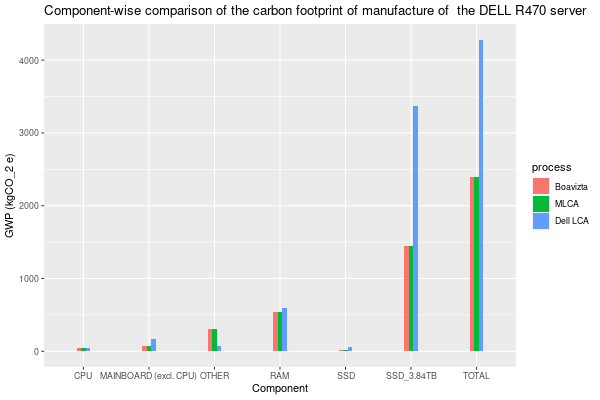
\includegraphics[width=.95\linewidth,page=1]{./figures/R470.png}                                                                                                                               
  \label{fig:R740}
  \caption{Component-wise comparison of the GWP of manufacture of the Dell R470 server}
\end{figure}


Figure \ref{fig:R740} compares the \gls{GWP} value obtained for the
different components by the boavizta tool, our tool (MLCA) and the
Dell \gls{LCA} result. As we can see, the boavizta tool and MLCA
obtain very close results. This is expected since MLCA is based on
Boavizta with some changes in the way CPU impacts are computed and
some bugfixes. We can see however that MLCA obtains a way lower
estimate than the expected results (Dell \gls{LCA}) but it seems to be
mainly explained by the difference in the estimate for the 3.84TB
SSDs. We can see that MLCA provides significantly lower estimates than
the expected result for these components. If we look at the server
without these big disks in figure \ref{fig:R740_no_SSD}, we can see that we obtain pretty close
estimates for the CPU, RAM and Total impacts with a lower estimate of
the impacts of the motherboard and an overestimate for the other
components that compensate a little.

\begin{figure}[t]
  \centering
  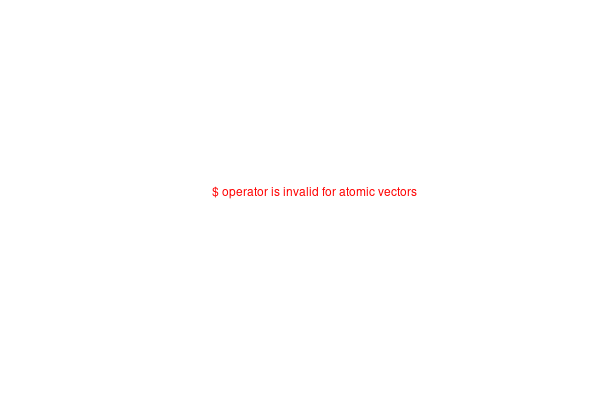
\includegraphics[width=.95\linewidth,page=1]{./figures/R470_no_SSD.png}                                                                                                                               
  \label{fig:R740}
  \caption{Component-wise comparison of the GWP of manufacture of the Dell R470 server not considering the 3.84TB SSDs}
\end{figure}


\subsection{Dell R6515, R7515, R6525, R7525}
\label{sec:orgf53f071}

In this section we compare the results our tool produces with
\gls{LCA} results produced by Sphera for Dell on the R6515, R7515, R7525
servers \cite{sphera2021lca}. Since there are few configuration differences
between the R6515 and R7515 and between the R6525 and R7525, we will
only focus on the R6515 and R6525.

First, we compare the total manufacture impact estimated by our tool
with the expected results : 

For the manufacture of the R6515, we obtain an estimate of 1200 kgCO\textsubscript{2}
e when the expected results stand at 1343 kgCO\textsubscript{2} e.
For the R6525, we obtain an estimate of 1600 kgCO\textsubscript{2} e when the expected
result stands at 1709 kgCO\textsubscript{2} e.

We can see that we obtain close results. If we now take a deeper look
at the repartition of impacts by components, Figure
\ref{fig:R6515_R6525} compares our tool (MLCA) with the expected
results from the Dell \gls{LCA}. As in section \ref{sec:R740}, we can
see that our tool underestimates the SSD impacts and produces a close
estimate of the total manufacture \gls{GWP} impact. We also see that
for the mainboard, we get a lower estimate that counterbalances the
overestimate for the other components. This time, the estimates for
the RAM and CPU impacts are farther from the expected result than in
the comparison for the Dell R470. Still, the overall results tend to
confirm the adequacy of the results our tool produces with expected
results about the manufacture impacts of a server.

\begin{figure}[t]
  \centering
  \begin{minipage}{.47\linewidth}
  \includegraphics[width=.95\linewidth,page=1]{./figures/R6515.png} 
  \end{minipage}
  \hspace{.06\linewidth}
  \begin{minipage}{.47\linewidth}
  \includegraphics[width=.95\linewidth,page=1]{./figures/R6525.png} 
  \end{minipage}                                                                                                                              
  \label{fig:R6515_R6525}
  \caption{Component-wise comparison of the GWP of manufacture for the Dell R6515 and R6525 servers}
\end{figure}


The comparison of our tool with the Dell \gls{LCA} results confirms
that overall, our tool produces adequate results component by
component even if it tends to
underestimate the impacts of storage. 

\section{replicating the Bloom estimates from \cite{Luccioni2022estimating}}
\label{sec:org32e8a1b}
\label{sec:bloom}
Now that we have tested our tool on the results it produces about the
energy consumption then on the manufacture impacts, let us test our
tool on all of this at the same time on the case of the Bloom carbon
footprint study.
\subsection{Gathering information about the setup}
\label{sec:org5ed1958}
To replicate their experiments, we first need to gather some
information on the time duration and hardware setup for the training
phase.

We can see in the paper that the training phase lasted for 118 days, 5
hours and 41 minutes for a total of 1,082,990 GPU hours. (table 1)

in section 4.1, we can read that training used on average 48 computing
nodes with 8 GPUs each.


Combining the real time and these information about the setup, we obtain an estimate of the number of GPU hours of 1,089,670.4 hours
this gives us a pretty close figure to the real GPU time.

It is written in the paper that training took place on the Jean Zay
supercomputer, using \href{https://buy.hpe.com/fr/fr/compute/apollo-systems/apollo-6500-system/apollo-6500-system/hpe-apollo-6500-gen10-plus-system/p/1013092236}{HPE's Apollo 6500 Gen10 Plus}. We can read on
their website that it uses AMD EPYC 7000 Series CPUs. Combining this
information with information about the Jean Zay supercomputer on
\href{http://www.idris.fr/jean-zay/cpu/jean-zay-cpu-hw.html\#gpu\_p13}{IDRIS's website}, we can see that only the \textbf{\textbf{gpu\textsubscript{p5}}}  partition uses
such CPUs. 
We can conclude that for each of the 48 used nodes, the server
configuration is :
\begin{itemize}
\item 2 CPUs : AMD Milan EPYC 7543
\item 512 Go of Memory
\item 8 NVIDIA A100 SXM4 80Go
\end{itemize}

\subsection{comparing the server footprint with the PCF sheet.}
\label{sec:orgd9d1305}

In section 4.1, it is stated that they use values provided in the
\href{https://www.hpe.com/psnow/doc/a50005151enw}{HPE ProLiant DL345 Gen10 Plus PCF}, the closest server with
information provided. In this PCF sheet, we can read that servers
are of type rack and that the estimated Carbon Footprint is of
2503.2 kg CO\textsubscript{2} e.

\begin{verbatim}
GWP: {'manufacture': 2300.0, 'use': 1170.0, 'unit': 'kgCO2eq'}
PE: {'manufacture': 29000.0, 'use': 39700.0, 'unit': 'MJ'}
ADP: {'manufacture': 0.17, 'use': 0.000198, 'unit': 'kgSbeq'}
RAM impact GWP: {'value': 1800.0, 'unit': 'kgCO2eq'}
\end{verbatim}


If we try our tool with the server configuration used for training, we
can see manufacture impacts of 2300 kg CO\textsubscript{2} e. This impact is close
to the 2500 kgCO\textsubscript{2} e provided on the PCF sheet and is mainly impacted
by the quantity of memory used, as it accounts for 1800 kg CO\textsubscript{2} e.

\subsection{comparing the GPU footprint with the chosen value}
\label{sec:orgc0de4b1}

In section 4.1 of the paper, it is stated that a value of 150 kg CO\textsubscript{2} e is
chosen. Taking a look at the source, there is no real justification
given for that value. Given that in \cite{Loubet2023life} a small GPUs
manufacture is estimated at emitting around 30 kg CO\textsubscript{2} e, we could
hypothesize that GPU manufacture impacts would be in the order of 50
to 150 kg CO\textsubscript{2} e.

For the specific model used, the "NVIDIA A100 SMX4 80GB", our tool
provides an estimate of 330 kgCO\textsubscript{2} e for the manufacture of one GPU. this impact is mainly influenced
by the quantity of memory on the GPU with a carbon footprint of 290
kgCO\textsubscript{2} e, leaving 40 kgCO\textsubscript{2} e for the rest of the GPU.
This estimate of 40kgCO\textsubscript{2} e for the GPU without any memory is
consistent with the values provided in \cite{Loubet2023life}. The
importance of the memory present on the GPU in its manufacture impacts
show the need for an \gls{LCA} of a modern GPU used for \gls{HPC} to
obtain good quality estimates


\subsection{Estimating the total impacts}
\label{sec:org32645dd}

with all of the previous information, we can run the estimation

with embodied impacts of 7T CO\textsubscript{2} e for the servers and 8.1T for the
GPUs to compare with the 7.6T for the servers and 3.6 T for the GPUs
in the paper. Most of the difference is due to estimated impacts of
330 kgCO\textsubscript{2} e for one GPU while it was estimated to 150 kgCO\textsubscript{2} e in the
paper.

For the dynamic consumption, we obtain an estimate of 23.7T CO\textsubscript{2} e,
mainly due to the GPUs (accountable for 22.4T, the only difference with
the figure obtained in the paper being the slightly off conversion
from real time to GPU hours) while the memory, not accounted for in
the paper brings another 1.35T CO\textsubscript{2} e.


\begin{table}[htbp]
\caption{Comparison of Estimated impacts with the expected impacts over the different sources of emissions}
\centering
\begin{tabular}{lrrrr}
Process & Expected CO\textsubscript{2} & Expected share & Estimated CO\textsubscript{2} & Estimated share\\
 &  & of total &  & of total\\
 & (TCO\textsubscript{2} e) & (\%) & (TCO\textsubscript{2} e) & (\%)\\
\hline
Embodied emissions & 11.2 & 22.2 & 15 & 25.4\\
Dynamic consumption & 24.69 & 48.9 & 23.7 & 40.2\\
Indirect consumption & 14.6 & 28.9 & 19.8 & 33.6\\
\hline
Total & 50.5 & 100 & 59 & 100\\
\end{tabular}
\end{table}

Table \ref{tab:bloom} compares  the results our tool produces on the
different sources of CO\textsubscript{2} emissions with the expected results.
As we can see, results for each category of emissions are pretty
similar even if we obtain a higher estimate for embodied emissions due
to a higher estimate of the manufacturing impacts of a GPU. More
surprisingly a higher Indirect consumption estimate than the one presented in
the paper estimate even if we are supposedly based on the same figures
to convert from dinamyc to Indirect consumption. This can be explained
by the fact that for an unknown reason, when presenting the results in
the paper, the authors did not talk about the Infrastructure consumption they
previously mentionned but only presented Idle consumptiion induced by
the Dynamic consumption.


\section{Conclusions}
\label{sec:org8ef1173}

After these experiments trying to evaluate the validity of our tool,
we can draw some conclusions, firstly about the challenges of
replicating results and then about the validity of our tool.

\subsection{about the replication of results}
\label{sec:orgc6667cc}

Overall, reproducing results from different papers proved way harder
than expected. Indeed, Unless a real effort is made by authors to allow replication of
their results, it is most of the time really difficult to find
enough information to run estimates and reproduce their
results.
This is also particularly true for results produced
using a measurement tool, indeed, If the hardware on which those
results were produced isn't detailed, it is impossible to
reproduce the experiments and check the quality of the results
presented. We were only able to conduct experiments for all of these
papers because we were able to contact the authors and they were
able to give us some insight about the hardware configuration of their experiments.

Even when we had enough information to run our estimates precisely
enough to hopefully match the expected results, we faced multiple
times important errors and inconsistencies in the data presented in
different tables. This was for example the case with the results
presented in \cite{Bannour2021evaluating} and in
\cite{Cattan2022benchmarking}. This was also the case to a lesser
extent in \cite{Jay2023experimental} were a notable effort for
reproducibility was realised by the authors but there were still
some problems and assumptions that needed to be made in order to
reproduce the results. 
After pointing out the problems with the data presented in
\cite{Cattan2022benchmarking}, the authors conducted new experiments
to resolve the problems with their data and we were able to reproduce
these new results.

\subsection{about the validity of the tool}
\label{sec:org09f822c}

Running new experiments often required us to gather some information
about a CPU not present in our database. This was not needed for
GPUs. It seems like there is much more diversity in CPUs used than in
GPU used. However, it was relatively easy to find all the information
we needed when encountering a new CPU and when running estimations
about GPU intensive tasks such as training NLP models, the CPU usage
is often set close to 0. Moreover, CPU manufacturing does not play a
huge part in the manufacturing impacts of a server in terms of
\gls{GWP}, it does however play an important part of the impacts in
terms of mineral resource usage (ADP)

We were unfortunately not able to find experiments to demonstrate the
validity of other indicators than the Global Warming Potential.

Still, we can see that overall, we were able to reproduce results for the
dynamic consumption and for the embodied impacts. These experiments
also demonstrate the usability of our tool in diverse scenarios.
\end{document}